\begin{apendicesenv}

%\partapendices

\chapter{Questionário de Pesquisa}
\label{ap:questionario}

Este apêndice apresenta o questionário de pesquisa (Tabela \ref{tab:quest-survey}), instrumento de coleta de dados usado na pesquisa com \textit{survey}. Esta é uma versão resumida, a versão completa encontra-se em: \url{https://github.com/RecursosDigitaisdeEnsinoAprendizagemIHC/research-pack-hci-games}.

\begin{table} [!h]
\centering
\caption{Perguntas do Questionário de Pesquisa}
\label{tab:quest-survey}
\begin{tabular}{|p{15.45cm}|}
\hline

\textbf{Seção 1} \\ \hline

I01 - Qual é a sua idade? \\ \hline

I02 - Qual o seu sexo? \\ \hline

I03 - Qual o nome da sua instituição de ensino? \\ \hline

I04 - Meu curso de graduação é da área Ciência da Computação? \\ \hline

\textbf{Seção 2} \\ \hline

O01 - Em relação à disciplina de Interação Humano-Computador (IHC):\\ \hline

H01 - Qual sua experiência com design de interfaces de software ou aplicativos?
\\ \hline


RL01 - O que você costuma fazer para sanar as dúvidas sobre algum conteúdo?
\\ \hline

O02 - Você já usou jogos para aprender algum conteúdo?\\ \hline

\textbf{Seção 3.1  } \\ \hline

O02.1.1 - Quais motivos levaram você a usar esse tipo de jogo? \\ \hline

O02.1.2 - Com qual frequência você usava esse tipo de jogo? \\ \hline

O02.1.3 - Cite alguns jogos para aprendizagem que você já utilizou? \\ \hline

O02.1.4 - Quais motivos levaram você a deixar de usar esse tipo de jogo? \\ \hline

\textbf{Seção 3.2 } \\ \hline

O02.2.1 - Quais motivos levaram você a usar esse tipo de jogo?\\ \hline

O02.2.2 - Com qual frequência você usava esse tipo de jogo?\\ \hline

O02.2.3 - Cite alguns jogos para aprendizagem que você  utiliza atualmente?\\ \hline

\textbf{Seção 3.3  } \\ \hline

O02.3.1 - Quais motivos levariam você a usar esse tipo de jogo?\\ \hline

O02.3.2 Por que você nunca usou esse tipo de jogo?
\\ \hline

\textbf{Seção 3.4} \\ \hline

O02.4.1 Por que você não tem interesse nesse tipo de jogo?\\ \hline

\textbf{Seção 4} \\ \hline

RE01  - Qual a relevância destes elementos para esse tipo de jogo?\tablefootnote{Os elementos da questão RE01  estão na Tabela \ref{tab:req-qualit}, com os indicadores de prioridade de 01 ao 12.} \\ \hline

E01 - Qual a importância destes elementos para uma boa experiência com estes jogos?\tablefootnote{Os elementos da questão E01 estão na Tabela \ref{tab:exp-player}, com os indicadores de prioridade de 01 ao 08.}\\ \hline

\end{tabular}
\legend{Fonte: Autor}
\end{table}

Este questionário segue uma lógica condicional a partir da questão O02 (Tabela \ref{tab:quest-survey}). Ao responder esta questão o respondente é encaminhado para uma seção distinta do questionário, de acordo com sua resposta. As opções da questão O02 são as seguintes: opção 1, ``Já usei, mas não jogo mais”, a qual o respondente é direcionado para questão O02.1.1 (Seção 3.1 da Tabela \ref{tab:quest-survey}); opção 2, ``Eu uso”, a qual o respondente irá continuar na questão O02.2.1 (Seção 3.2 da Tabela \ref{tab:quest-survey}); opção 3, ``Não uso, mas tenho interesse em jogar”, a qual o respondente segue para questão O02.3.1 (Seção 3.3 da Tabela \ref{tab:quest-survey}); e a opção 4, ``Não uso e não tenho interesse em jogar”, a qual ele é direcionado para O02.4.1 (Seção 3.4 da Tabela \ref{tab:quest-survey}). 

Depois de seguir para uma determinada seção, o respondente segue o fluxo de perguntas da respectiva seção. Dependendo de qual esteja, ao responder a algumas destas questões O02.1.4, O02.2.3, O02.3.2 ou O02.4.1, ele é direcionado à ultimação seção do questionário, partindo da questão RE01 (Seção 4 da Tabela \ref{tab:quest-survey}).


%-------------------Tabela RQ -------------------

Na questão RE01 o respondente classifica alguns elementos de acordo com sua relevância nos jogos. Na Tabela \ref{tab:req-qualit} são apresentados estes elementos, os requisitos de qualidade apreciados pelos jogadores referentes aos item da questão RE01 da Tabela \ref{tab:quest-survey}. 

\begin{table}[htbp]
\centering
\caption{Requisitos de Qualidade Apreciados pelos Jogadores}
\label{tab:req-qualit}
\begin{tabular}{|p{1cm}|p{9cm}|p{1.5cm}|}
\hline
\textbf{ID}& \textbf{Requisito de Qualidade} & Fonte \\ \hline
01             & \textit{Design} do jogo atraente & PW, SS\\ \hline
02             & Padrão de \textit{design} consistente & PW\\ \hline
03             & Facilidade em aprender a jogar & PW, SS  \\ \hline
04             & Facilidade em jogar & PW  \\ \hline
05             & Regras fáceis e claras de se entender & PW \\ \hline
06             & Fontes usadas serem fáceis de ler & PW \\ \hline
07             & Uso adequado das cores & PW \\ \hline
08             & Acessibilidade & PW \\ \hline
09             & Oferece \textit{feedback} ao jogador  & SS \\ \hline
10             & Possui uma narrativa ou história  &  SS \\ \hline
11             & Oferece pontos e recompensas  & SS \\ \hline
12             & Apresenta \textit{ranking} dos jogadores & SS \\ \hline

\multicolumn{3}{|c|}{
Legenda: SS - \citeonline{deSales_SousaeSilva_2020}; PW - \citeonline{Petri_Wangenheim_2019}} \\ \hline
\end{tabular}
\legend{Fonte: Autor} 
\end{table}

%-------------------Tabela PX -------------------

Estes são os requisitos não funcionais, originários do trabalho de \citeonline{deSales_SousaeSilva_2020}, identificados pela legenda SS (Tabela \ref{tab:req-qualit}) e os fatores de usabilidade do modelo MEEGA+ \cite{Petri_Wangenheim_2019}, identificados pela legenda PW (Tabela \ref{tab:req-qualit}).

\newpage

Já na questão E01 o respondente classifica mais alguns outros elementos de acordo com sua importância nos jogos. Na Tabela \ref{tab:exp-player} são apresentados estes elementos, as experiências apreciadas pelo jogador referentes aos item da questão E01 da Tabela \ref{tab:quest-survey}.

\begin{table}[htbp]
\centering
\caption{ Experiência Apreciada pelos Jogadores}
\label{tab:exp-player}
\begin{tabular}{|p{1cm}|p{8.5cm}|p{1.5cm}|}
\hline
\textbf{ID} & \textbf{Experiência apreciada pelos jogadores} & Fonte \\ \hline
1                 & Ter confiança de que aprenderei o conteúdo & PW  \\ \hline
2                 & Me sentir desafiado        &  PW, SS        \\ \hline
3                 & Sentir satisfação em jogar e aprender & PW, SS \\ \hline
4                 & Interagir com outros jogadores    &   PW, SS     \\ \hline
5                 & Me divertir           &   PW, SS             \\ \hline
6                 & Ter a atenção focada durante o jogo    &  PW    \\ \hline
7                 & Perceber a relevância do conteúdo ensinado & PW   \\ \hline
8                 & O jogo como o principal meio de aprendizagem  & PW  \\ \hline
\multicolumn{3}{|c|}{
Legenda: SS - \citeonline{deSales_SousaeSilva_2020}; PW - \citeonline{Petri_Wangenheim_2019}} \\ \hline
\end{tabular}
\legend{Fonte: Autor}                                       
\end{table}

Estas são as experiências de usuário, apresentadas no trabalho de \citeonline{deSales_SousaeSilva_2020}, identificados pela legenda SS (Tabela \ref{tab:req-qualit}) e os fatores de experiência do jogador do modelo MEEGA+ \cite{Petri_Wangenheim_2019}, identificadas pela legenda PW (Tabela \ref{tab:req-qualit}).

%nas Figuras \ref{Fig:survey1.png}, \ref{Fig:survey2.png} e \ref{Fig:survey3.png}.

% \begin{figure}[htbp]
% 	\centering
% 	\subfigure[Questionário Parte 1]{
%         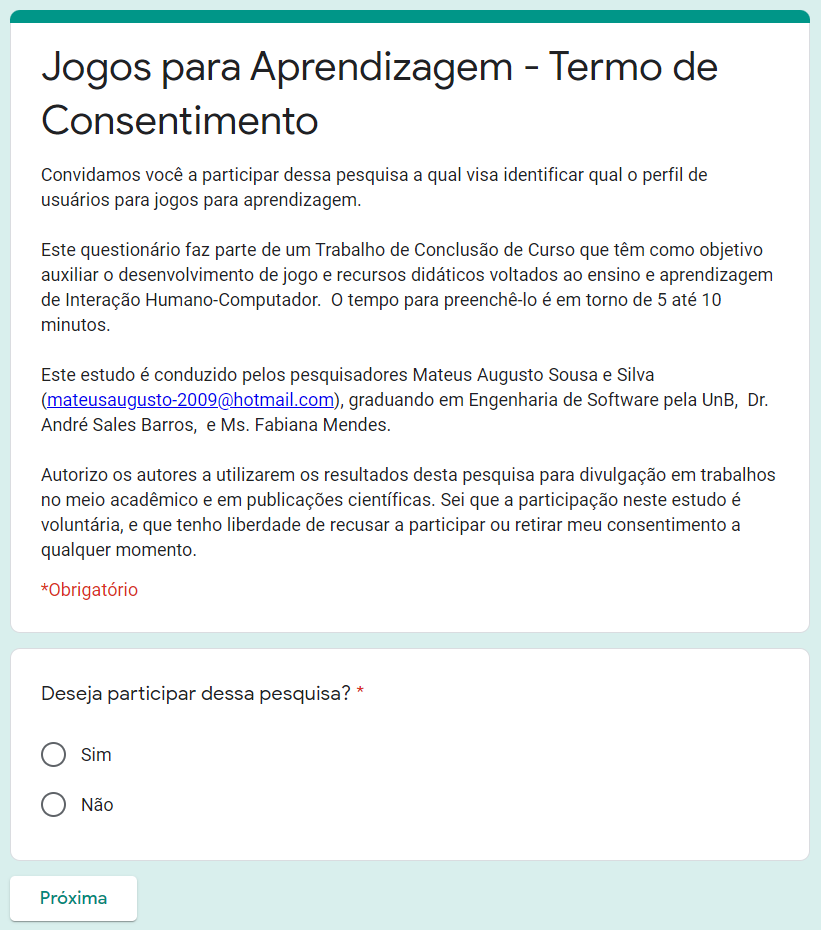
\includegraphics[keepaspectratio=true,scale=0.325]{figuras/apendice/Capture.PNG}
%         \label{Fig:survey_pt1.png}
%     }
%     \quad
%     \subfigure[Questionário Parte 2]{
%         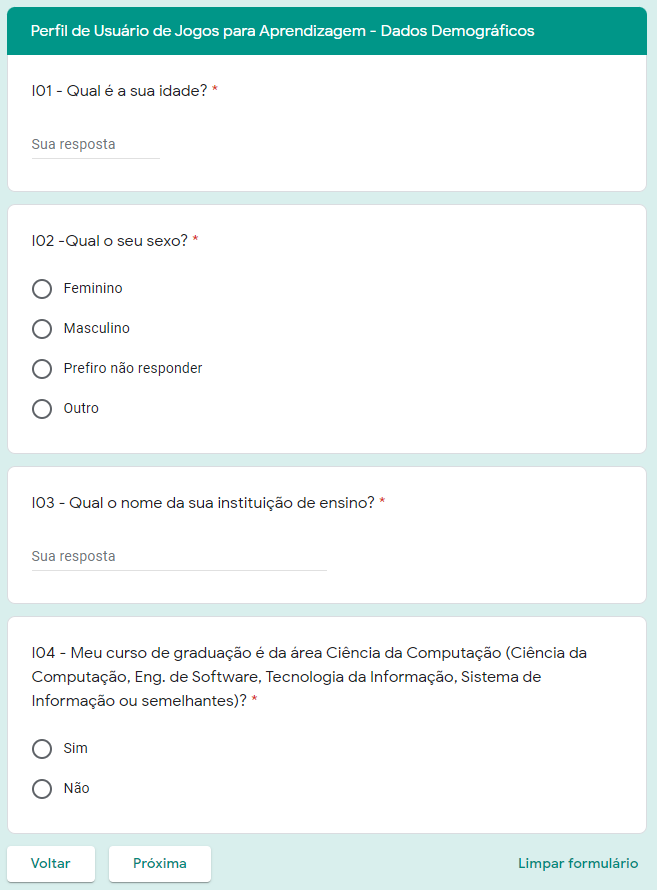
\includegraphics[keepaspectratio=true,scale=0.325]{figuras/apendice/Capture1.PNG}
%         \label{Fig:survey_pt2.png}
%     }
%     \quad
%      \subfigure[Questionário Parte 3]{
%         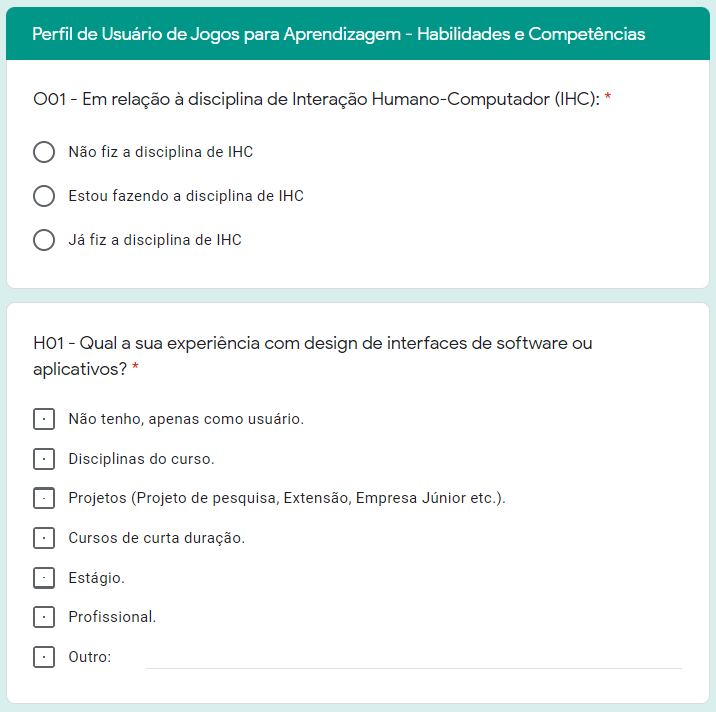
\includegraphics[keepaspectratio=true,scale=0.325]{figuras/apendice/Capture2.PNG}
%         \label{Fig:survey_pt3.png}
%     }
%     \quad
%      \subfigure[Questionário Parte 4]{
%         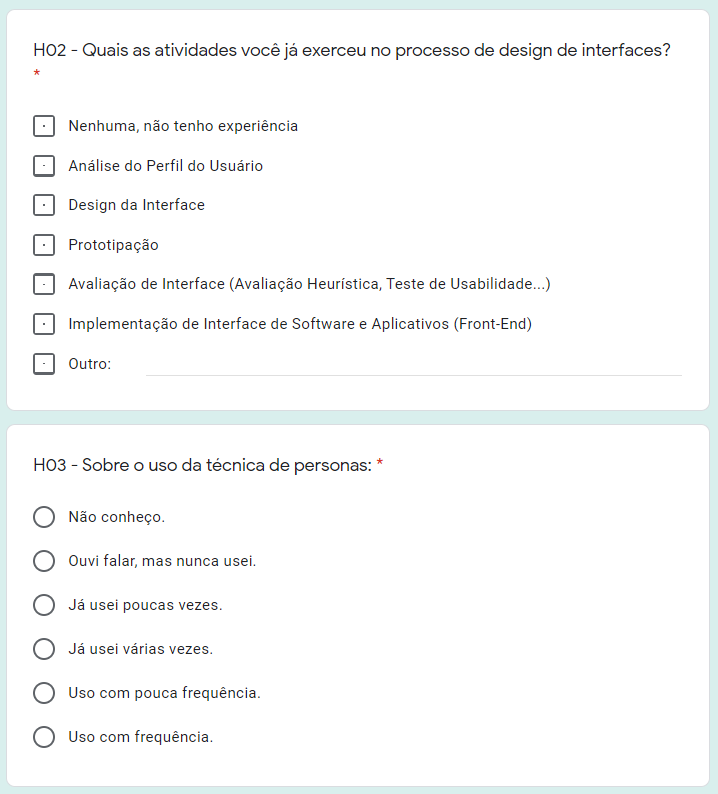
\includegraphics[keepaspectratio=true,scale=0.325]{figuras/apendice/Capture3.PNG}
%         \label{Fig:survey_pt4.png}
%     }
   
% 	\caption{Questionário de Pesquisa da Parte 1 à 4 - Fonte: Autoral}
% 	\label{Fig:survey1.png}
% \end{figure}

% \begin{figure}[htbp]
% 	\centering
% 	\subfigure[Questionário Parte 5]{
%         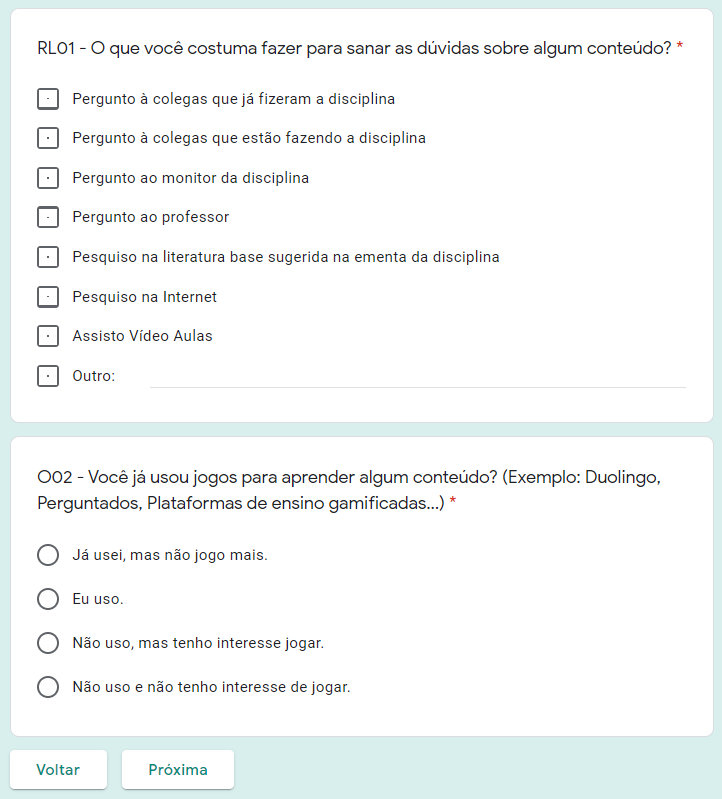
\includegraphics[keepaspectratio=true,scale=0.325]{figuras/apendice/Capture4.PNG}
%         \label{Fig:survey_pt5.png}
%     }
%     \quad
%     \subfigure[Questionário Parte 6]{
%         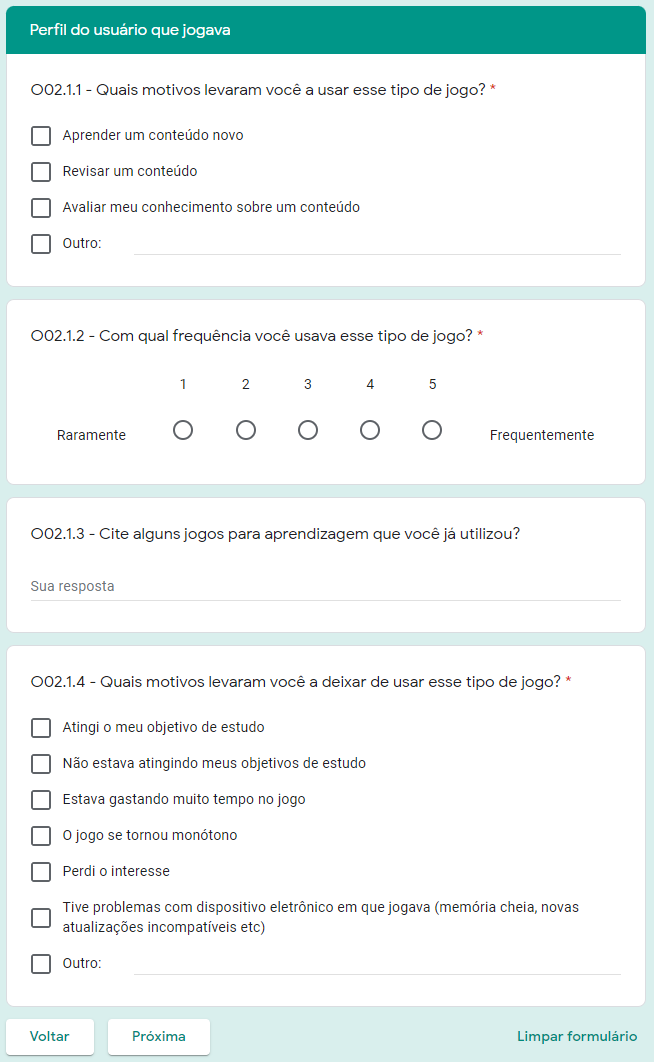
\includegraphics[keepaspectratio=true,scale=0.325]{figuras/apendice/Capture5.PNG}
%         \label{Fig:survey_pt6.png}
%     }
%     \quad
%      \subfigure[Questionário Parte 7]{
%         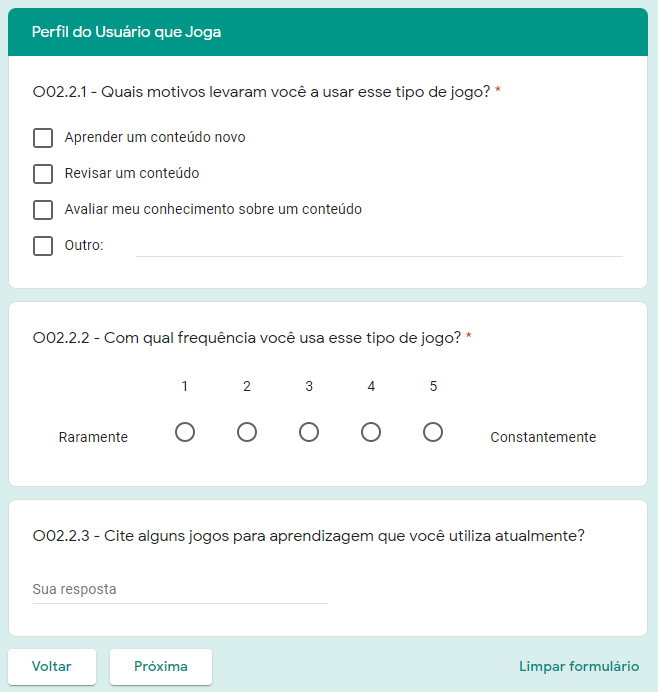
\includegraphics[keepaspectratio=true,scale=0.325]{figuras/apendice/Capture6.PNG}
%         \label{Fig:survey_pt7.png}
%     }
%     \quad
%      \subfigure[Questionário Parte 8]{
%         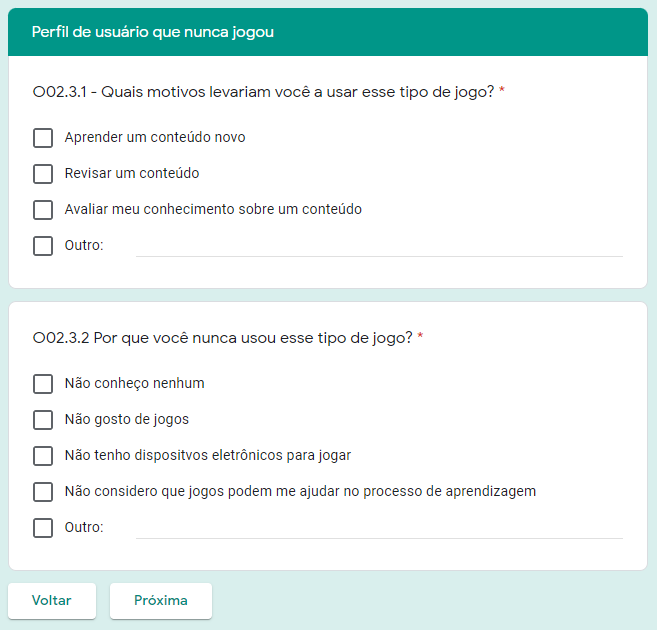
\includegraphics[keepaspectratio=true,scale=.325]{figuras/apendice/Capture7.PNG}
%         \label{Fig:survey_pt8.png}
%     }
   
% 	\caption{Questionário de Pesquisa da Parte 5 à 8 - Fonte: Autoral}
% 	\label{Fig:survey2.png}
% \end{figure}

% \begin{figure}[htbp]
% 	\centering
% 	\subfigure[Questionário Parte 9]{
%         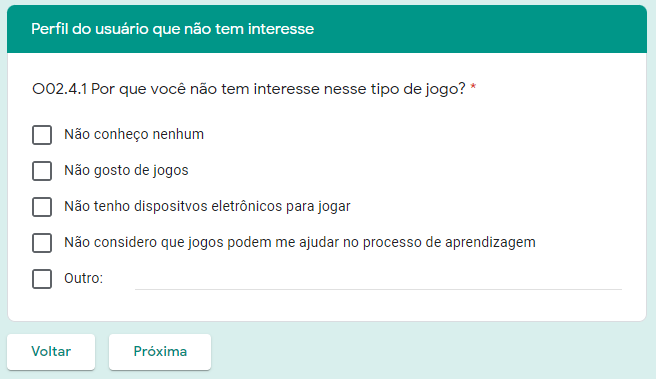
\includegraphics[keepaspectratio=true,scale=0.325]{figuras/apendice/Capture8.PNG}
%         \label{Fig:survey_pt9.png}
%     }
%     \quad
%     \subfigure[Questionário Parte 10]{
%         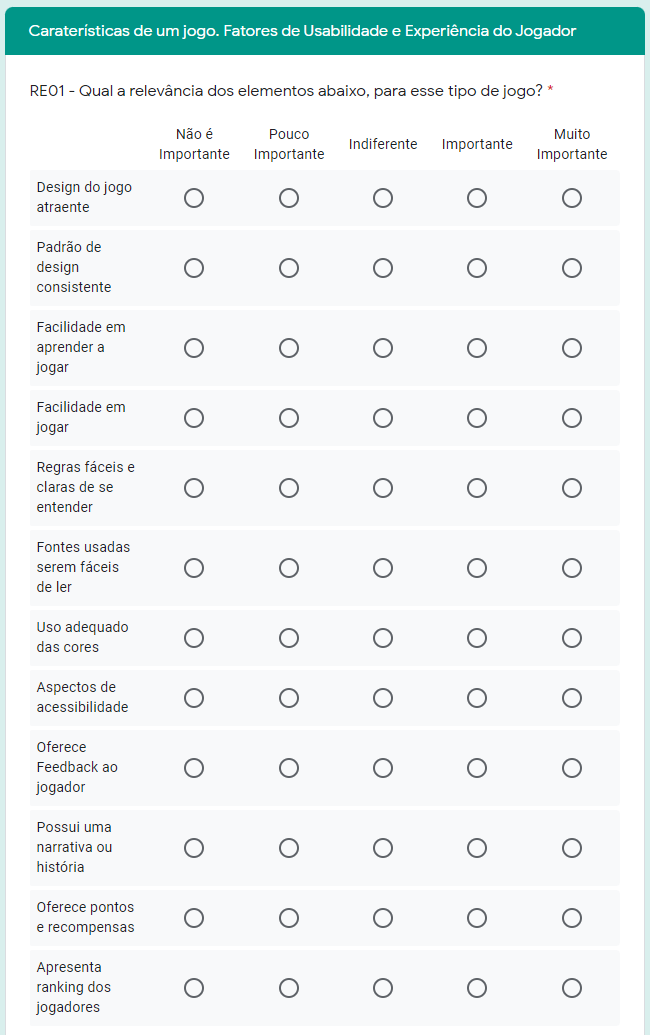
\includegraphics[keepaspectratio=true,scale=0.325]{figuras/apendice/Capture9.PNG}
%         \label{Fig:survey_pt10.png}
%     }
%     \quad
%      \subfigure[Questionário Parte 11]{
%         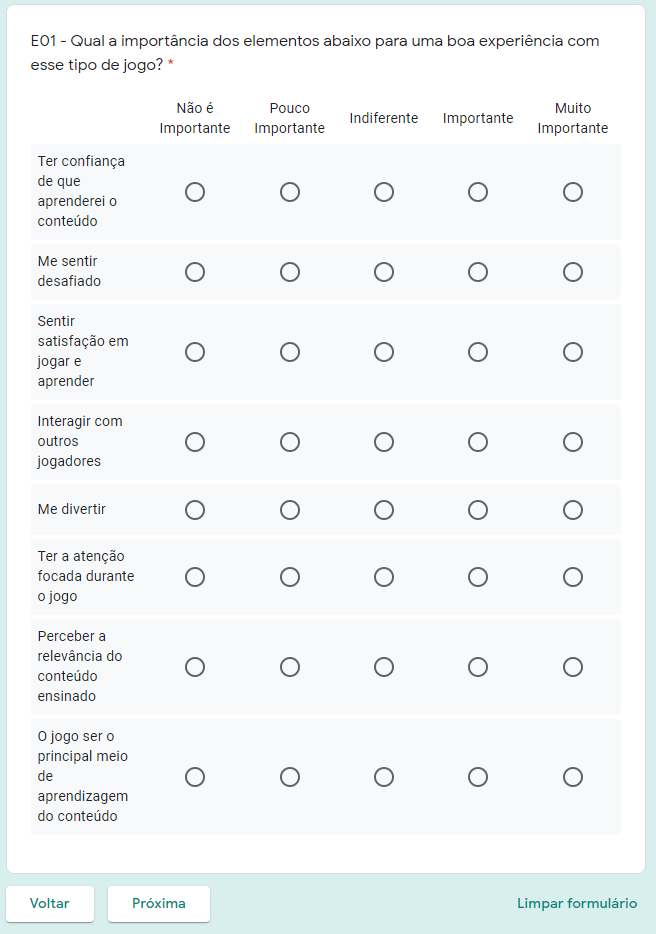
\includegraphics[keepaspectratio=true,scale=0.325]{figuras/apendice/Capture10.PNG}
%         \label{Fig:survey_pt11.png}
%     }
%     \quad
%      \subfigure[Questionário Parte 12]{
%         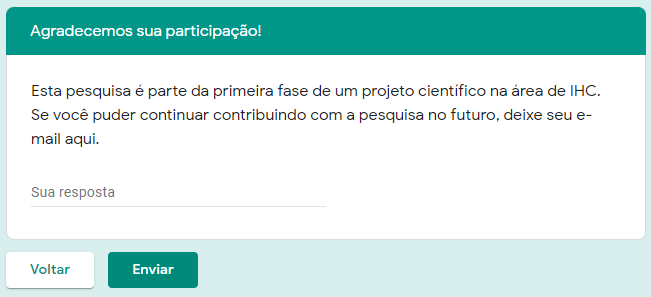
\includegraphics[keepaspectratio=true,scale=0.325]{figuras/apendice/Capture11.PNG}
%         \label{Fig:survey_pt12.png}
%     }
   
% 	\caption{Questionário de Pesquisa da Parte 9 à 12 - Fonte: Autoral}
% 	\label{Fig:survey3.png}
% \end{figure}


\end{apendicesenv}